\documentclass[../FinalThesis.tex]{subfiles}
\begin{document}
\chapter{General Introduction}
\label{GeneralIntroduction}
\thispagestyle{empty}
\vspace{-1cm}
\noindent\hfil\rule{0.75\textwidth}{.4pt}\hfil

\newpage

% \section{Thesis Outline}

% This thesis consists of seven chapters; a general introduction, four data
% chapters, a chapter about additional works, and a general discussion.  In the
% general introduction, I introduce the general background and research topics of
% this thesis. In particular, I discuss the importance of dispersal and
% connectivity in the context of conservation science and highlight multiple
% limitations in current connectivity research. I also introduce the study system
% and give a brief overview of the data collection and general research methods.
% In chapters two to four, I investigate and address several limitations of
% current connectivity research. In chapter five, I outline some additional works
% that I have conducted or co-supervised. Finally, in the general discussion, I
% summarize my findings and embed them in a broader context. I also provide an
% outlook for topics that require further research, and provide conservation
% insights for the African wild dog.
% \newpage

\section{Ecological Networks in the Anthropocene}

Life on earth is in constant motion. Birds migrate seasonally between their
summering and wintering grounds from the Northern to the Southern Hemisphere
\citep{Alerstam.1993}, humpback whales (\textit{Megaptera novaeangliae})
traverse thousands of kilometers to gather at breeding sites
\citep{Rasmussen.2007}, monarch butterflies (\textit{Danaus plexippus}) relocate
from their summer habitats in North America to their winter roosts in Mexico in
a multi-generational journey \citep{Reppert.2018}, and zebras (\textit{Equus
quagga}) and wildebeest (\textit{Connochaetes taurinus}) participate in one of
nature's most spectacular migrations, traversing from the southern Serengeti in
Tanzania to the Masai Mara in Kenya \citep{Serneels.2001}. If there wasn't any
movement, there wouldn't be any life. Life is movement, and movement is life.

Although life on Earth has thrived in motion for millennia, we have entered an
era of decline \citep{IPBES.2019, Almond.2022}. The beginning of the
Anthropocene \citep{Crutzen.2006} not only cemented the domination of humanity
over nature \citep{Kareiva.2007, Johns.2022}, but also heralded a sixth mass
extinction event \citep{Barnosky.2011, Ceballos.2015}. With the current
extinction rate surpassing the background rate by several orders of magnitude
\citep{Ceballos.2015, Ceballos.2017}, approximately 1 million species are at the
brink of extinction \citep{IPBES.2019}. This rapid decline in biodiversity can
mainly be attributed to an ever-expanding human footprint and a continued
exploitation of natural resources \citep{Venter.2016, Ceballos.2017}. To date,
18\% of the Earth's land is heavily modified, 56\% is less severely transformed,
and only 26\% remain unaffected and intact \citep{Locke.2019}. The loss of
formerly healthy habitats and their fragmentation into isolated patches not only
reduces biodiversity directly but also entails a reduction in species ability to
roam freely \citep{Haddad.2015}, thus limiting their capacity to cope with
altered climatic conditions via range shifts \citep{Fahrig.2003, Heller.2009,
Chen.2011, Tucker.2018}. The need for conservation action is evident and urgent.

In order to slow or even reverse the biodiversity loss, many countries have
taken conservation measures and established or expanded protected areas
\citep{Bingham.2021}. Besides the direct protection of endangered ecosystems
through protection zones, the identification and preservation of major movement
corridors that provide connectivity and promote dispersal between remaining
areas is a prominent conservation strategy \citep{Fahrig.2003, Doerr.2011,
Rudnick.2012}. By linking national parks, wildlife management areas, and other
biodiversity hotspots, connectivity shifts conservation from small isolated
``wildlife islands'' to transboundary ecological networks \citep{Hilty.2020}.
Within these networks, animals can again roam freely, allowing them to overcome
resource scarcity, re-colonize extinct patches, and track suitable habitat
conditions. The ability to move and disperse thus crucially contributes to
population viability, stressing the importance of preserving and enhancing
dispersal and connectivity, especially in light of anticipated challenges due to
climate change \citep{Heller.2009}.

\section{Dispersal}

Dispersal of individuals, i.e., the movement of individuals away from their
natal range to the site of first reproduction, is an important process governing
the dynamics of spatially distributed species \citep{Howard.1960, Clobert.2012}.
By moving individuals from one area to another, dispersal constitutes the main
mechanism by which connectivity among subpopulation arises and can be maintained
\citep{Fahrig.2003}. Dispersal differs from migration in that dispersing
individuals do not seasonally move between known patches, but venture into areas
they are unfamiliar with \citep{Hundertmark.2007}. This promotes the
colonization of vacant habitats \citep{Gustafson.1996, Hanski.1999,
MacArthur.2001} and facilitates the reinforcement of small and nonviable
subpopulations \citep{Brown.1977}. Because dispersing individuals (hereafter
referred to as dispersers) cross an inhospitable matrix more willingly than
resident individuals (hereafter residents), they help to offset some of the
negative consequences of habitat-fragmentation by moving between otherwise
isolated habitats \citep{Marsh.2004, Elliot.2014}. At a macro-evolutionary
scale, dispersal enhances range expansions and enables species to track suitable
environmental conditions under climate change \citep{Kokko.2006, Hodgson.2012,
Hodgson.2016}. Finally, dispersal plays a central role in maintaining gene-flow,
thus facilitating adaptation and promoting metapopulation viability and
resilience \citep{Brachet.1999, Marsh.2004, Heinz.2006}. Overall, dispersal
reduces the risk of stochastic extinctions \citep{Shaffer.1985, Melbourne.2008},
making it a key element of many conservation strategies \citep{Baguette.2013}.

\section{Connectivity}

A species' ability to disperse hinges on a sufficient amount of landscape
connectivity \citep{Doerr.2011}. Connectivity is typically defined as the degree
to which a landscape facilitates or impedes movement of organisms among resource
patches \citep{Taylor.1993}, and can be subdivided into \textit{structural} and
\textit{functional} connectivity \citep{Tischendorf.2000}. Structural
connectivity is primarily focused on the size and configuration of habitat
patches within the landscape. It is therefore considered an inherent property of
the landscape that is independent of the focal species, thus overlooking many of
the interesting but complex interactions between organisms and their
environment. Under a \textit{functional} connectivity perspective, conversely,
the focal species' behavioral response to prevailing environmental conditions is
taken into account \citep{Tischendorf.2000}. A landscape with similar structural
properties can thus result in vastly different patterns of functional
connectivity depending on the species of interest. In functionally
well-connected landscapes, species can effectively migrate, disperse, forage,
and establish new populations. Together, these processes contribute to the
resilience, functioning, and diversity of natural systems, and, ultimately,
sustain life on Earth. Preserving functionally connected landscapes has
therefore become the gold-standard in conservation management
\citep{Heller.2009, Doerr.2011, Rudnick.2012}.

\section{Modeling Connectivity}

Although dispersal and connectivity have fascinated and interested scientists
for decades, they both remained notoriously difficult to study until recently.
Dispersers only make up a small fraction of an entire population, and the
proximate causes of dispersal are seldom known (but see \citealp{Behr.2020}).
This makes it challenging to select appropriate individuals and to predict the
exact moment they will emigrate, thus resulting in modest sample sizes, even for
large studies \citep{Nathan.2001, Rudnick.2012, Fattebert.2015}. Following
dispersers is also logistically challenging, due to animals leaving well-defined
study areas and crossing national borders. This holds particularly true for
species that disperse over vast distances \citep{Osipova.2019, Elliot.2014,
Cozzi.2020}. The choice of data and an appropriate connectivity model is
therefore often driven by data availability \citep{Baguette.2013} and frequently
lacks biological justification \citep{Sawyer.2011, Zeller.2012}. Furthermore,
connectivity studies usually cover extensive spatial extents, requiring coherent
environmental data at very large spatial and temporal scales. Thanks to the
uprise and miniaturization of automated tracking devices, the task of monitoring
dispersal has become less problematic, allowing to remotely follow the fate of
dispersing individuals \citep{Cagnacci.2010, Kays.2015, Jonsson.2016,
Williams.2019, Nathan.2022}. Simultaneously, an increased availability of remote
sensed satellite products allows obtaining environmental data at the necessary
spatio-temporal scale to link observed dispersal movements to habitat
characteristics \citep{Toth.2016, Rumiano.2020}.

Thanks to the rapid increase in data-availability on both species and
landscapes, various modeling techniques to quantify connectivity have emerged
(see e.g. \citealp{Etherington.2016} and \citealp{Diniz.2019} for reviews,
\Cref{ConnectivityModeling}). Early approaches were limited to examining
structural aspects of connectivity, focusing on the composition and
configuration of habitat patches, while ignoring the focal species' response to
environmental conditions \citep{Doerr.2011, Diniz.2019}. With the uprise of
tracking data and novel methods to study species' habitat and movement
preferences (\citealp{Boyce.2002, Fortin.2005, Cushman.2010, Avgar.2016,
Fieberg.2021}), however, the focus has shifted towards a more functional view,
taking into account how species react to prevailing habitat conditions
\citep{Diniz.2019}. Presently, the most prominent functional connectivity models
are based on least-cost path analysis (LCPA; \citealp{Adriaensen.2003}), circuit
theory (CT; \citealp{McRae.2006, McRae.2008}) and individual-based movement
models (IBMMs; \citealp{Kanagaraj.2013, Allen.2016, Hauenstein.2019,
FletcherJr..2019, Zeller.2020, UnnithanKumar.2022, FletcherJr..2023}). LCPA and
CT are graph-based methods that estimate conductance of the landscape, whereas
IBMMs use simulations to quantify connectivity. LCPA attempts to identify
least-costly routes between predefined start and endpoints, whereas CT assumes a
random walk and uses laws from electrical circuit theory to calculate
conductance through each area of the landscape. Notably, LCPA and CT are linked
via a concept coined \textit{randomized} LCPA, which allows deviations (the
degree of which can be specified by the user) from the least-costly route, thus
approximating a random walk \citep{Panzacchi.2016}. Except for a few IBMMs, all
functional connectivity models require a permeability surface as an input
\citep{Diniz.2019}. This surface is a spatial raster layer indicating the
expected ease or difficulty at which the focal species can traverse a specific
area given the area's environmental characteristics \citep{Adriaensen.2003,
Zeller.2012}. Permeability can be gauged from expert opinion or using empirical
data, yet the latter approach has proven more accurate \citep{Clevenger.2002,
Zeller.2012}, especially when GPS data are available \citep{Elliot.2014,
Graves.2014, Gaston.2016, Jackson.2016, Keeley.2017}. Unfortunately, due to the
limited availability of dispersal data, most studies utilize data collected on
resident individuals (e.g., \citealp{Brennan.2020, Lines.2021}), despite the
perception and motivation of dispersing and resident individuals to cross
landscape features is arguably different \citep{Elliot.2014, Benz.2016}. Popular
approaches to empirically parametrize permeability surfaces are
resource-selection functions \citep{Fortin.2005, Manly.2007, Thurfjell.2014,
Cushman.2010}, which estimate habitat preferences of the focal species by
comparing used habitat to available habitat \citep{Zeller.2012}. For GPS data,
the use of integrated step-selection functions (iSSFs) has proven particularly
useful, as they readily account for the autocorrelation inherent to GPS data
\citep{Fortin.2005, Avgar.2016}.

\begin{figure}[htpb]
\begin{center}
  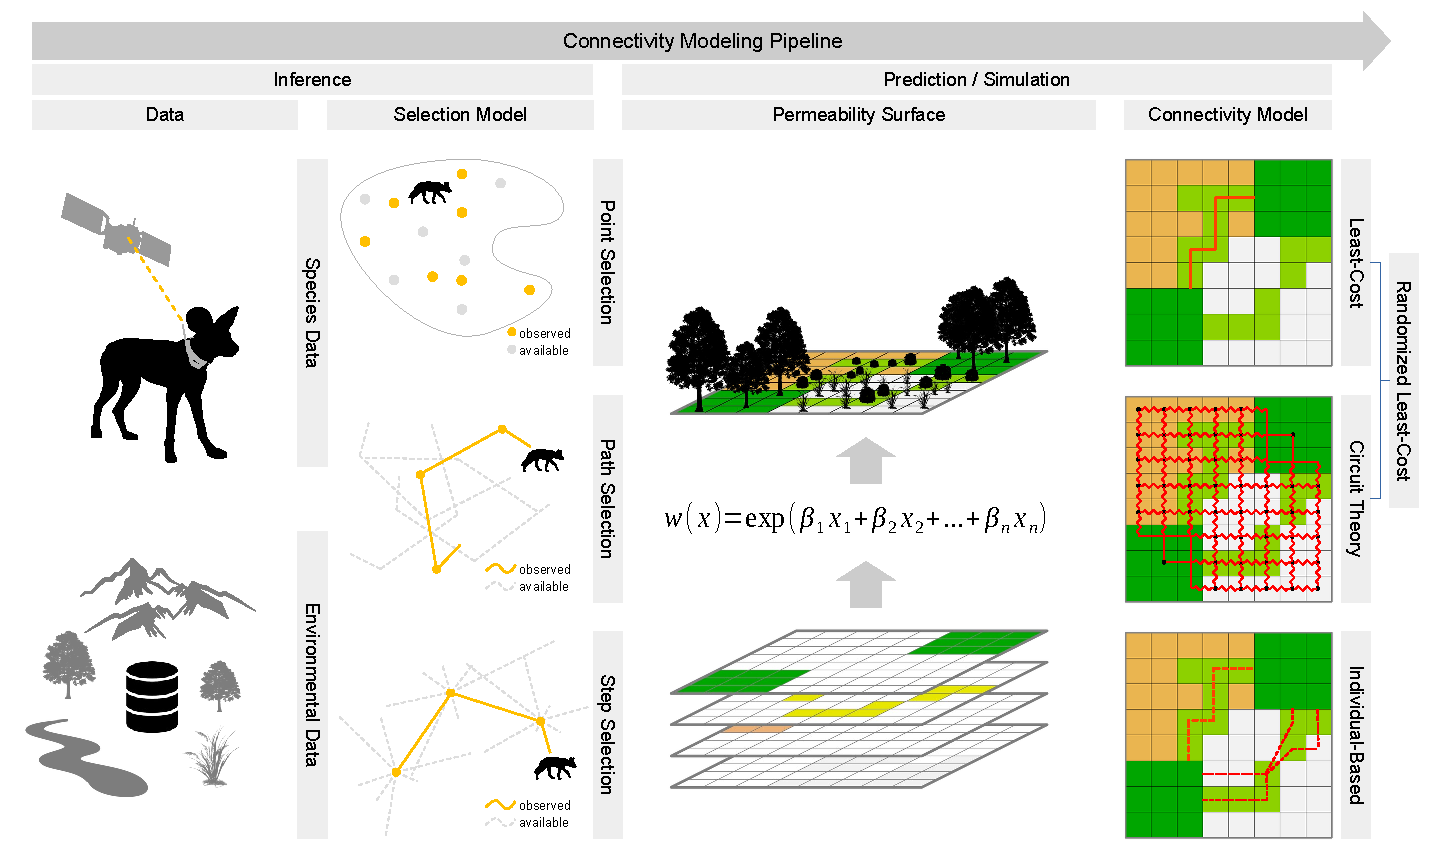
\includegraphics[width = \textwidth]{Figures/ConnectivityModeling}
  \caption{Conceptualized illustration of a typical connectivity modeling
  pipeline. The pipeline typically starts by collection information on the focal
  species, as well as on environmental features believed to influence the
  species' movement. In a next step, this data is paired and fed into a
  selection model, which empirically estimates selection or avoidance towards
  different landscape conditions. Most frequently, this is achieved via point-
  (or home-range) selection functions, path-selection functions, and
  step-selection functions \citep{Zeller.2012}. Estimated preferences (here
  denoted $\beta$) are then used to predict a permeability surface, indicating
  the expected ease or difficulty at which the modeled species can traverse each
  grid-cell in the landscape, given that grid-cell's covariate values. Finally,
  the permeability surface is used as an input to a connectivity models.
  Currently, least-cost models and circuit theory are among the most prominent
  connectivity models, yet individual-based have been employed as well
  \citep{Diniz.2019}. Figure adapted from \citet{Zeller.2012} and
  \citet{Diniz.2019}.}
  \label{ConnectivityModeling}
\end{center}
\end{figure}

\section{Limitations of Current Approaches}

Despite significant advances in the realms of modeling dispersal and
connectivity, important limitations remain. For my master's thesis, I applied
iSSFs to parametrize a permeability surface and employed LPCA to identify major
movement corridors for dispersing African wild dogs \citep{Hofmann.2021}. This
work exposed me to several of the existing limitations and sparked the
motivation for some of the chapters of this PhD thesis.

\subsection{Use of Traditional Connectivity Models}

A first limitation concerns the use of traditional LCPA and CT (e.g.,
\citealp{Elliot.2014, Mallory.2019, Brennan.2020}), which both make assumptions
that are rarely met by dispersers. LCPA, for instance, assumes that dispersers
have perfect knowledge about their target location and associated movement
costs, allowing them to find the least-costly route. CT, conversely, presumes
that individuals follow a random walk and are ignorant of their target location.
Furthermore, both methods hinge on a permeability surface, which is an
\textit{unconditional} prediction of permeability and cannot render that an
animal's decision to disperse across a certain habitat is contingent on what
else is available \citep{Signer.2017}. IBMMs are a promising alternative that
eliminate the need for a permeability surface \citep{Signer.2017, Diniz.2019,
UnnithanKumar.2022} and enable more realistically rendering an animal's
landscape perception \citep{Zeller.2020a, Zeller.2020}. However, a unified
framework for the parametrization and application of IBMMs to estimate
connectivity is missing.

\subsection{The Assumption of Static Landscapes}

A second limitation in current connectivity analyses lies in their exclusive
focus on present environmental conditions without consideration of how climate
change could affect on-the-ground conditions and therefore species' ability to
disperse (but see \citealp{Ashrafzadeh.2019} and \citealp{Luo.2021}). Yet, an
emphasis on present rather than future environmental conditions might lead to
misguided conservation recommendations in light of ongoing climate change. The
ability to model how climate change affects landscape connectivity would
therefore be highly valuable. A similar limitation arises from the use of static
environmental data, which provide only a snapshot in time and, consequently,
overlook spatio-temporal variations in connectivity due to seasonality
\citep{Simpkins.2017a, Zeller.2020a}. Since most ecosystems experience
significant seasonal changes in environmental conditions, it can be anticipated
that connectivity is not a static property and should be modeled dynamically.
Since incorporating seasonality entails substantial complexity, the question
then becomes to what degree seasonality should enter connectivity analyses to
still distill meaningful conservation insights \citep{Zeller.2020a}.

\subsection{Data Irregularity}

Finally, a last and more technical limitation relates to the use of iSSFs. iSSFs
are regularly used in connectivity modeling to obtain species-specific habitat
preferences and movement capacities (or movement preferences) from GPS location
data \citep{Avgar.2017, Fieberg.2021}. For the method to work, GPS data need to
be collected at regular temporal intervals, which in reality is rare due to GPS
devices occasionally failing to obtain a location. The current practice of
removing irregular data can result in substantial losses of data, which can have
negative consequences, especially in cases where data are already scarce.
Alternatives that allow coping with slightly irregular data would therefore be
desirable.

\section{Thesis Goals}

My goal with this thesis is to address the above outlined limitations and, where
applicable, to provide methodological alternatives. I will do so using
dispersing African wild dogs from the Okavango Delta area in northern Botswana
as a study system. This system lends itself to examine the described limitations
for several reasons. Firstly, the African wild dog is among the world's most
wide-ranging species and a species of immediate conservation concern. The study
population in Botswana is considered a stronghold population that likely acts as
a source for the recolonization of surrounding areas \citep{Cozzi.2013a,
Cozzi.2020}. Furthermore, the African wild dog exemplifies a species that
crucially depends on dispersal and transboundary connectivity for population
viability (cfr. \Cref{StudySpecies}). Because the study area in Botswana
undergoes significant seasonal changes \citep{Mendelsohn.2010} and is among the
most vulnerable to climate change \citep{Akinyemi.2019, IPCC.2022}, it also
offers a unique opportunity for studying the impacts of seasonality and climate
change on connectivity (cfr. \Cref{StudyArea}).

\section{Study Species}
\label{StudySpecies}

The African wild dog (henceforth abbreviated as AWD, \textit{Lycaon pictus}) is
a medium-sized canid native to Sub-Saharan Africa and the only extant
representative of its genus \citep{Kingdon.2015}. It is recognized by its
individually distinct, tricolored coat pattern and large ears (\Cref{WildDog}).
The AWD is a highly social animal, forming packs comprising 5 to 15 adult
individuals that operate as cohesive units \citep{Kuhme.1965, Frame.1979}.
Established packs exhibit a well-defined social structure, with a dominant pair
monopolizing the majority of reproduction and subordinates helping to rear pups
\citep{Frame.1979}.

Once widespread across Sub-Saharan Africa (\Cref{GeneralStudyArea}a), AWDs have
disappeared from a vast majority of their historic range. This decline is mainly
traced back to deadly diseases, human persecution, and habitat destruction
\citep{Fanshawe.1991, Woodroffe.2020}. With fewer than 6,000 individuals
remaining in the wild, the IUCN categorizes the AWD as endangered
\citep{Woodroffe.2020}. The biggest continuous population remains in northern
Botswana, which is the main study area of this research project. AWDs occupy
vast home-ranges, encompassing between 200 km\textsuperscript{2} and 2,000
km\textsuperscript{2} \citep{Pomilia.2015}. Due to their need for vast,
undisturbed spaces, AWDs are particularly vulnerable to habitat fragmentation
and have become an umbrella species for conservation efforts across sub-Saharan
Africa \citep{Dalerum.2008, Brennan.2020}. AWDs thus offer a unique opportunity
for studying transboundary connectivity.

AWDs are crepuscular to diurnal hunters \citep{Saleni.2007}, active primarily
during the cooler morning and evening hours \citep{Kuhme.1965, Creel.2001}, as
well as during moonlit nights \citep{Estes.1967, Saleni.2007, Cozzi.2012}. With
a lean and athletic build, they are exceptionally well-adapted to endurance
hunting \citep{Taylor.1971, Estes.1967, Koshy.2020, Smith.2020}, allowing them
to chase prey until exhaustion \citep{Estes.1967, Creel.1995, Rhodes.2004}. In
the focal study area, packs mainly hunt by means of opportunistic and individual
chases \citep{Hubel.2016}. They predominantly predate on medium-sized antelopes,
including impala (\textit{Aepyceros melampus}) and kudu (\textit{Tragelaphus
strepsiceros}), but occasionally take smaller quarry, such as warthogs
(\textit{Phacochoerus africanus}) and steenbok (\textit{Raphicerus campestris},
\citealp{Creel.1995, Mills.1997, Hayward.2006, Tshimologo.2021}).

Across the majority of their range, AWDs coexist and compete with stronger
competitors, especially with lions (\textit{Panthera leo}) and spotted hyenas
(\textit{Crocuta crocuta} \citealp{Creel.2001, Cozzi.2012, Vogel.2019,
Creel.2023}). To evade potentially fatal encounters, AWDs avoid both species
temporally and spatially \citep{Creel.1996, Cozzi.2012, Droge.2017},
particularly during the denning season \citep{VanDerMeer.2013, Mbizah.2014,
Jackson.2014, Davies.2016, Alting.2021}. The displacement of AWDs by stronger
competitors may explain why the species occurs predominantly in areas of
intermediate prey density \citep{Mills.1997, Mbizah.2014, Creel.2002,
Creel.2023}.

Upon reaching sexual maturity (1.5 to 3 years of age), individuals disperse from
their natal pack in an attempt to find potential mates and a suitable territory
to settle \citep{McNutt.1996, Behr.2020}. Both sexes disperse, typically in
same-sex sibling coalitions comprising two to five members \citep{Frame.1979,
McNutt.1996, Behr.2020}. On average, dispersing AWDs cover Euclidean distances
between 5 and 500 km \citep{Davies-Mostert.2012, Masenga.2016, Cozzi.2020,
Sandoval-Seres.2022}, yet cumulative distances up to 5,000 km have been reported
\citep{Masenga.2016}. Studies on habitat-selection suggest that dispersing AWDs
avoid areas covered by water and dominated by humans, but prefer open shrubs and
grassland \citep{Cozzi.2020, ONeill.2020, Hofmann.2021}. During dispersal, their
movements are characterized by fast, directional bursts away from their natal
location \citep{Cozzi.2020, Hofmann.2021}.

\begin{figure}[htpb]
\begin{center}
  \includegraphics[width = \textwidth]{Figures/WildDogPoster}
  \caption{(a) An adult African wild dog photographed in northern Botswana. The
  distinct fur markings are unique to each individual. (b) An anesthetized wild
  dog is being equipped with a GPS/Satellite collar, allowing to remotely follow
  its movements. (c) An African wild dog chasing prey at high speed.}
  \label{WildDog}
\end{center}
\end{figure}

\section{Study Area}
\label{StudyArea}

Data on dispersing AWDs were collected in northern Botswana as part of a
collaborative effort between the Botswana Predator Conservation Program (BPC)
and the University of Zurich. BPC was founded in 1989, when John Weldon ``Tico''
McNutt commenced his pioneering work on AWDs in Botswana and established a
research station \citep{Fuller.1992, McNutt.1996, Osofsky.1996}. The program has
continued ever-since, making it the longest running research program on AWDs and
resulting in invaluable long-term data (e.g., \citealp{McNutt.1996, Cozzi.2012,
Broekhuis.2013, Abrahms.2016, Behr.2020, Jordan.2022}).

BPC's historic study area (approx. 3,000 km\textsuperscript{2}, centered at
19\degree 31'S, 23\degree 38'E, \Cref{GeneralStudyArea}b) is located at
the Eastern fringes of the world-renowned Okavango Delta, a flood-pulse driven
mosaic of patchy woodlands, permanent swamps, and seasonally flooded grasslands
that lie within the otherwise dry and sandy Kalahari Basin \citep{Wilson.1976,
Ramberg.2006, Mendelsohn.2010}. The Okavango Delta represents the world's
largest inland delta and is classified as a Ramsar site, supporting a rich
ecosystem with diverse flora and fauna. Precipitation in this area is highly
seasonal and limited to the wet-season between October and April. Rainwater is
collected in the Angolan highlands and only slowly descends through the Okavango
Delta's tributaries into its alluvial fan, so the flood is out of sync with
local rains and reaches its maximum extent during peak dry season in July-August
\citep{Wolski.2017}.

Human influence across the study area remains low, with large portions of land
being gazetted national parks, wildlife management areas, or other protected
areas. The study area is also part of the Kavango-Zambezi Transfrontier
Conservation-Area (KAZA-TFCA, \Cref{GeneralStudyArea}a), the world's largest
transboundary conservation initiative. The KAZA-TFCA was initially aimed towards
restoring connectivity for migrating elephants (\textit{Loxodonta africana}),
but has gained momentum as an opportunity to establish connectivity for several
other wide-ranging species, including the African wild dog \citep{Brennan.2020,
Hofmann.2021, Sandoval-Seres.2022}.

\begin{figure}[htpb]
\begin{center}
  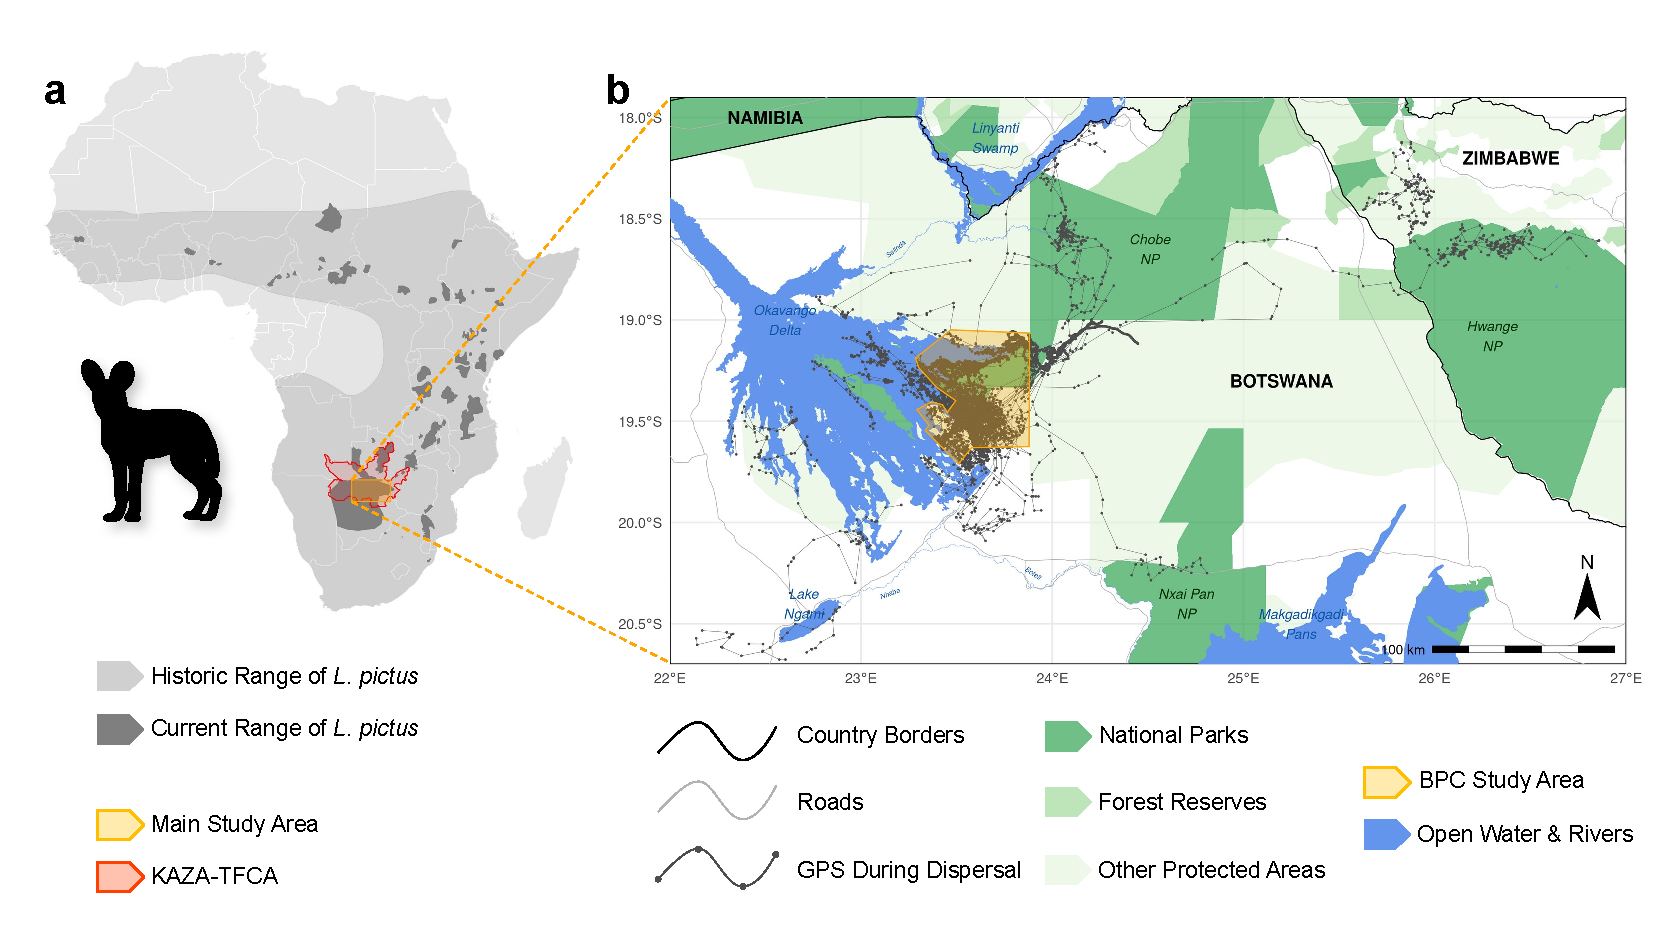
\includegraphics[width = \textwidth]{Figures/GeneralStudyArea.pdf}
  \caption{(a) The main study area of this thesis is located in northern
  Botswana and forms part of the world's largest transboundary conservation
  initiative, the Kavango-Zambezi Transfrontier Conservation Area (KAZA-TFCA).
  (b) Within this area, Botswana Predator Conservation (BPC) has continuously
  monitored a core area, spanning about 3,000 km\textsuperscript{2}. The
  dominant geographical feature of this ecosystem is the Okavango Delta, a flood
  pulse driven conglomerate of diverse habitats. Dispersers were collared within
  BPC's main study area and moved into various regions, including the Chobe
  National Park in Botswana and the Hwange National Park in Zimbabwe.}
  \label{GeneralStudyArea}
\end{center}
\end{figure}

\section{General Methods}

\subsection{Data Collection}

GPS data on dispersing AWDs were collected between 2011 and 2023 using
GPS/Satellite collars (Vertex Lite; Vectronic Aerospace GmbH, Germany).
Candidate dispersing individuals were selected based on age, number of same-sex
siblings, pack size and presence of unrelated individuals of the opposite sex in
their pack \citep{McNutt.1996, Behr.2020}. Following the procedure described by
\citet{Osofsky.1996}, selected individuals were immobilized using a mixture of
ketamine and xylazine, which was subsequently reversed with yohimbine. Drugs
were injected through a dart shot from a CO\textsubscript{2}-pressurized
dart-gun (Dan-Inject, Denmark) at distances ranging from 10-12 m. During
anesthesia, collars were attached, body measurements recorded, and blood samples
collected. After 45 minutes, the anesthesia was reversed and the animal's
recovery was monitored until it rejoined its pack. All required procedures were
conducted by a Botswana-registered wildlife veterinarian, and all dispersers
were collared while they were still with their natal pack. Deployed collars
weighed about 330 g ($\approx$ 1\% of the species' body weight) and contained a
decomposable mechanism that ensured drop-off of the collar after 12–18 months.
Collars were programmed to record a GPS location every 4 hours during dispersal,
and to regularly transmit data via Iridium satellite system to a base station.
To distinguish between residency and dispersal in the recorded data, I relied on
a combination of data collected in the field and visual inspection of the
net-squared displacement metric. Net-squared displacement measures the squared
Euclidean distance of a location to a reference point \citep{Borger.2012}, which
I set at the center of the dispersing wild dog's natal range. Thus, I deemed
dispersal to have started when an individual left its pack and natal range, and
I defined settlement once the net-squared displacement metric flattened off.
Besides GPS data on dispersers, I compiled an extensive collection of data on
environmental conditions (e.g. water cover, human influence, temperature)
sourced through publicly available services, or remote sensed from free
satellite imagery. Specific details about additional data will be introduced in
the relevant chapters.

I completed all processing steps and analyses using R \citep{RCoreTeam.2023} and
performed computations exclusively on a desktop PC with AMD Ryzen 7 2700X
octa-core processor (8 x 3.6 GHz, 16 threads) and 64 GB DDR4 RAM. All
\texttt{R}-scripts and \LaTeX files associated with this thesis are available
through GitHub (\url{https://github.com/DavidDHofmann/PhD}).

\subsection{Statistical Analyses}

Throughout all chapters, I heavily rely on the framework of iSSFs. I therefore
briefly summarize the method here. iSSFs are frequently applied in movement
ecology to study an animal's habitat preferences and movement capacity
\citep{Fortin.2005, Thurfjell.2014, Avgar.2016}. They operate in discrete time
and mathematically model the probability $u$ of finding an individual at a
location $s$ at time $t+1$, given the animal's past positions at time $t$ and
$t-1$, $s_t$ and $s_{t-1}$. Formally, this probability is given by:

\begin{equation}
\label{EQ0}
u(s_{t+1}) = \frac{\phi(s_{t+1}, s_t, s_{t-1}; \gamma)w(x(s_{t+1}); \beta)}{\int_{s \in G}\phi(s_{t+1}, s_{t}, s_{t-1}; \gamma)w(x(s_{t+1}); \beta)ds}
\end{equation}

\noindent The function $\phi$ represents an animal's movement kernel which is
usually expressed in terms of a step-length and turning-angle distribution, with
$\gamma$ representing parameters in these distributions (for simplicity, I will
sometimes refer to the \textit{movement kernel} as \textit{movement
preferences}). The function $w$ defines the habitat-selection function and
reflects an animal's preferences $\beta$ towards environmental characteristics
$x$ at location $s_{t+1}$. In most applications, $w$ is defined as the
log-linear function $w = exp(x^\top\beta)$. Finally, the integral in the
denominator of \ref{EQ0} ensures that $u$ is a proper probability distribution
and integrates to one.

To estimate parameters in \ref{EQ0} using empirical data, one needs to convert
observed GPS locations into sequences of temporally regularly-spaced steps.
Here, a step is defined as the straight line connecting two consecutive GPS
locations \citep{Turchin.1998} and is characterized by a step length, absolute
turning angle (a.k.a. heading), and relative turning angle. The likelihood in
\ref{EQ0} can then be maximized by comparing observed steps with random steps in
a (mixed effects) conditional logistic regression model (\citealp{Fortin.2005,
Muff.2020}, but see \citealp{Michelot.2016} for alternatives). The required
random steps can be generated by sampling step lengths and turning angles from
parametric distributions fitted to empirical data \citep{Fortin.2005,
Thurfjell.2014}.

To jointly estimate parameters in $\phi$ and $w$, movement descriptors (e.g.,
step length (sl), its natural logarithm (log(sl)), and the cosine of the turning
angle (cos(ta))) can be included in the regression model, and their estimated
coefficients serve to update the tentative parameters of the step-length and
turning-angle distributions \citep{Duchesne.2015, Avgar.2016, Fieberg.2021}. By
including the relevant predictors, iSSFs allow modeling highly complex movement
behaviors (e.g., \citealp{Munden.2021, Forrest.2024}). Notably, a model fitted
using iSSFs constitutes a mechanistic movement model from which movement can be
simulated \citep{Avgar.2016, Signer.2017, Signer.2024}.

\section{Thesis Outline}

This thesis comprises six chapters; a general introduction, four data chapters,
and a general discussion. All published chapters of this thesis are verbally
reproduced as they appeared in the respective journals, including personal
pronouns, jargon, and abbreviations. References cited in each chapter are
listed at the end of the thesis.

% In the general introduction, I introduce the general background and research
% topics. In particular, I discuss the importance of dispersal and connectivity in
% the context of conservation science and highlight multiple limitations in
% current connectivity research. I also introduce the study system and give a
% brief overview of the data collection and general research methods.

% In chapters two to four, I investigate and address several limitations of
% current connectivity research. In chapter five, I outline some additional works
% and supervised thesis. Finally, in the general discussion, I summarize my
% findings and embed them in a broader context. I also provide an outlook for
% topics that require further research, and provide conservation insights for the
% African wild dog.

In \Cref{ChapterSimulation}, I present a novel simulation approach to study
landscape connectivity via simulated dispersal. Specifically, I introduce a
simple three-step approach to quantify landscape connectivity using IBMMs,
starting from empirical dispersal data and a set of landscape layers. The
simulation approach relies on iSSFs, which enable a detailed representation of
dispersers' habitat and movement preferences. In contrast to traditional
connectivity modeling techniques, this approach bypasses the need for a
permeability surface and overcomes several important limitations, such as the
assumption that dispersers move towards a predefined endpoint. To translate
simulated dispersal trajectories into meaningful measures of functional
connectivity, I propose three complementary connectivity metrics, each focused
on a different aspect of connectivity. This includes a heatmap, revealing
frequently traversed areas, a betweenness map, highlighting critical movement
corridors, and a map of inter-patch connectivity, summarizing dispersal
frequencies and durations. I demonstrate the application of the approach using
dispersing AWDs in the KAZA-TFCA as a case-study. I thereby show how landscape
connectivity varies across the KAZA-TFCA landscape and reveal critical movement
corridors. This chapter was published in \textit{Landscape Ecology} in 2023
(\url{https://doi.org/10.1007/s10980-023-01602-4}).

In \Cref{ChapterFlood}, I study functional connectivity for AWDs in light of
increasingly extreme climatic conditions due to climate change. Specifically, I
study how climate-induced changes to the Okavango Delta's flooding regime could
influence AWDs' ability to move between remaining populations. For this, I
compile over 20 years of remote sensed satellite data on flood conditions and
derive two extreme scenarios that serve to approximate flood conditions under
climate change. For both scenarios, I simulate AWD dispersal and investigate
emerging connectivity patterns. I show that periods of increased flooding result
in isolated subpopulations and reduced dispersal prospects. Conversely, I find
that periods of reduced floods reveal vast dispersal habitats that can be used
to transfer from one subpopulation to another. Overall, this work highlights the
importance of accounting for anticipated on-the-ground conditions in light of
climate change when assessing landscape connectivity. This chapter was published
in \textit{Global Change Biology} in 2024
(\url{https://doi.org/10.1111/gcb.17299}).

In \Cref{ChapterSeasonality}, I investigate the importance of accounting for
seasonal dynamism when investigating landscape connectivity. To do so, I first
provide a conceptual framework to motivate that seasonality can enter
connectivity analyses at multiple stages; when (1) extracting spatial covariates
for model fitting, (2) when fitting the selection model, and (3) when making
predictions from the fitted model. Via combination, this provides six distinct
configurations that differ in their amount of dynamism. Using GPS data on
dispersing AWDs, I parametrize the models associated with each configuration and
employ a rigorous validation approach to assess at which stages rendering
seasonality is critical. I also employ IBMMs to simulate dispersal under varying
degrees of seasonal dynamism and examine the emerging patterns of connectivity.
Notably, in the most dynamic configuration, I update seasonal covariates as the
simulated dispersers move; a similar degree of seasonality cannot be achieved
via traditional approaches. Even though the validation procedure reveals only a
marginal benefit of increasing dynamism, I find that emerging patterns of
connectivity differ markedly depending on the level of incorporated dynamism.
Specifically, a static approach results in more clumped dispersal hotspots,
whereas a dynamic take suggests more heterogeneously distributed dispersal
movements. This chapter highlights that the predictive improvements reaped by
incorporating seasonality into connectivity analyses may be moderate, despite
marked differences in inferred patterns of connectivity.

In \Cref{ChapterIrregularity}, I revisit the iSSF framework utilized throughout
Chapters 2 to 4. A major drawback of iSSFs is that they presume that GPS data
were collected at regular time intervals, whereas in reality GPS data are often
incomplete and gappy, thus exhibiting slight irregularities between successive
GPS locations. Usually, such irregular data need to be removed, implying a
substantial reduction in effective sample size. To overcome this limitation, I
introduce and compare several methods that account for irregularity, thereby
allowing to retain additional GPS data for modeling. I use simulations with
known parameters to compare the effectiveness of different methods and show that
irregularity can be effectively accounted for when appropriate methods are used.
I also exemplify the application of the best performing method to a case study
using GPS data on a spotted hyena. The divergence from using AWD dispersal data
was primarily due to the availability of an extensive dataset on a single
spotted hyena. This chapter was published in \textit{Movement Ecology} in 2024
(\url{https://doi.org/10.1186/s40462-024-00476-8}).

% In \Cref{AdditionalWorks}, I give a brief overview of additional works that I
% have conducted during my PhD and summarize two master theses that I have
% co-supervised.

Finally, in \Cref{GeneralDiscussion}, I synthesize and reflect on the main
insights of this thesis and discuss how this work integrates into the existing
literature. I also elaborate on some of the methodological and biological
implications of my work, with a particular focus on conservation insights for
the African wild dog. Finally, I highlight potential limitations and give an
outlook for future research.

\ifSubfilesClassLoaded{%
  \newpage
  \begin{singlespacing}
  \ifthenelse{\boolean{usebiblatex}}{
    \begin{refcontext}[sorting=nyt]
    \printbibliography
    \end{refcontext}
  } {
    \bibliography{../LiteratureBibtex}%
  }
\end{singlespacing}
}{}

\end{document}
